\documentclass[12pt]{article}
\usepackage[margin=1.0in]{geometry} %page layout
\usepackage[usenames,dvipsnames]{color} %color
\definecolor{light-gray}{gray}{0.95}
\definecolor{darkgreen}{rgb}{0,0.4,0}
\usepackage{graphicx, subfigure} %figures
\usepackage{url, hyperref} %cross-referencing
\usepackage{amsmath, amssymb} %math
\usepackage{listings} %source code
\lstset{breaklines=true,
breakindent=0pt,
prebreak=\mbox{\tiny$\searrow$},
postbreak=\mbox{{\color{blue}\tiny$\rightarrow$}},
numbers=left,
commentstyle=\color{darkgreen},
numberblanklines=false,
frame=single,
captionpos=b,
backgroundcolor=\color{light-gray}}
\usepackage[3D]{movie15} %for movies (needs hyperref)
\author{Salman Aslam\\Georgia Tech}
\title{RVQ Tree Entanglement}
\author{Salman Aslam\\ Georgia Institute of Technology}
\date{}
\definecolor{darkgreen}{rgb}{0,0.5,0}
\newcommand{\Ntrg}{\big[N_{t=1, m=1} + \lambda \big] + \big[N_{t=1, m=2} + \lambda \big] + \ldots + \big[N_{t=1, m=M} + \lambda \big]}
\newcommand{\jointcnt}{\sum\limits_{n_{trg}=1}^{N_{trg}}I(X_t=x_t, X_{t-1}=x_{t-1})}
\newcommand{\singlecnt}{\sum\limits_{n_{trg}=1}^{N_{trg}}I(X_{t-1}=x_{t-1})}
\newcommand{\singlep}{p(X_{t-1}=x_{t-1})}
\newcommand{\singlepone}{p(X_{t-1}=1)}
\newcommand{\singleptwo}{p(X_{t-1}=2)}
\newcommand{\singlepM}{p(X_{t-1}=M)}
\newcommand{\condp}{p(X_t=x_t | X_{t-1}=x_{t-1})}
\newcommand{\jointp}{p(X_t=x_t, X_{t-1}=x_{t-1})}
\newcommand{\KmeansOuterSum}{\sum\limits_{k=1}^K}
\newcommand{\KmeansInnerSum}{\sum\limits_{{i=1 \atop x_i \in \mathcal{K}_k}}^N}
\newcommand{\KmeansSum}{\KmeansOuterSum \KmeansInnerSum}
\newcommand{\RVQInnerSum}{\sum\limits_{{i=1 \atop g_i \mapsto m_{\tau, s}}}^N}
\newcommand{\RVQOuterSum}{\sum_{s=1}^S}
\newcommand{\RVQsum}{\KmeansOuterSum \sum\limits_{{i=1 \atop g_i \in \mathcal{K}_k}}^N}
\newcommand{\KmeansInner}{{(x_i - \mu_k)}^2}
\newcommand{\RVQinner}{            {(x_i  - \hat{\mu}^{(k)})}^2}
\newcommand{\RVQinneralternate}{{(g_i - m_\tau^{(k)})}^2}
\newcommand{\RVQinneralternatealternate}{{(g_i - m_{\tau, s})}^2}
\newcommand{\KmeansError}{\KmeansSum \KmeansInner}
\newcommand{\RVQerror}     {\KmeansSum \RVQinner}
\newcommand{\RVQerroralternate}{\RVQsum \RVQinneralternate}
\newcommand{\RVQunit}{x_i -\bigg(\sum_{t=1}^Tm^{(k)}_t\bigg)}
\newcommand{\RVQequivalentCodevector}{\sum_{t=1 }^Tm^{(k)}_t}
\newcommand{\RVQequivalentCodevectorBroken}{\sum_{t=1 \atop t \neq \tau}^Tm^{(k)}_t+ m^{(k)}_\tau}
\newcommand{\RVQmultipleKmeans}{x_i -\bigg(\RVQequivalentCodevectorBroken\bigg)}
\newcommand{\RVQmultipleKmeansone}{x_i -\sum_{t=2}^Tm^{(k)}_t+ m^{(k)}_1\bigg)}
\newcommand{\RVQmultipleKmeansonealternate}{\bigg(x_i -\sum_{t=1 \atop t \neq \tau}^Tm^{(k)}_t\bigg) - m^{(k)}_\tau}
\newcommand{\RVQmultipleKmeanstwo}{x_i -\bigg(\sum_{t=1 \atop t \neq 2}^Tm^{(k)}_t+ m^{(k)}_2\bigg)}
\newcommand{\RVQmultipleKmeansT}{x_i -\bigg(\sum_{t=1}^{T-1}m^{(k)}_t+ m^{(k)}_2\bigg)}
\newcommand{\EucMatrix}
{
\left[
\begin{array}{lll}
r_{11} & r_{12} & t_x \\ 
r_{21} & r_{22} & t_y \\ 
0 & 0 & 1 \\ 
\end{array}
\right]
}	

\newcommand{\SimMatrix}
{
\left[
\begin{array}{lll}
sr_{11} & sr_{12} & t_x \\ 
sr_{21} & sr_{22} & t_y \\
0 & 0 & 1 \\ 
\end{array}
\right]
}

\newcommand{\AffMatrix}
{
\left[
\begin{array}{lll}
a &b & t_x \\ 
c & d & t_y \\
0 & 0 & 1 \\
\end{array}
\right]
}

\newcommand{\ProjMatrix}
{
\left[
\begin{array}{lll}
h_{11} & h_{12} & h_{13} \\ 
h_{21} & h_{22} & h_{23} \\ 
h_{31} & h_{32} & h_{33} \\ 
\end{array}
\right]
}

\newcommand{\RotMatrixTheta}
{
\left[
\begin{array}{rr}
\cos(\theta) & -\sin(\theta) \\ 
\sin(\theta) & \cos(\theta) \\ 
\end{array}
\right]
}

\newcommand{\RotMatrixPhi}
{
\left[
\begin{array}{rr}
\cos(\phi) & -\sin(\phi) \\ 
\sin(\phi) & \cos(\phi) \\ 
\end{array}
\right]
}

\newcommand{\RotMatrixminusPhi}
{
\left[
\begin{array}{rr}
\cos(-\phi) & -\sin(-\phi) \\ 
\sin(-\phi) & \cos(-\phi) \\ 
\end{array}
\right]
}


\newcommand{\EigenvalueMatrix}
{
\left[
\begin{array}{cc}
\lambda_1 & 0\\
0 & \lambda_2
\end{array}
\right]
}

\newcommand{\bigMatrix}
{
s \left[
\begin{array}{cc}
 (r)(a) + b &  (r)(d) - c \\
 (r)(c) - d &  (r)(b) + a
\end{array}
\right]
}


\newcommand{\bigMatrixTwo}
{
\left[
\begin{array}{cc}
(\lambda_2) p + (\lambda_1) q & (\lambda_2) s  - (\lambda_1) r \\
(\lambda_2) r  - (\lambda_1) s & (\lambda_2) q + (\lambda_1) p
\end{array}
\right]
}
\newcommand{\dr}{(\mathbf{x}_i-\boldsymbol\mu_k)^T(\mathbf{x}_i-\boldsymbol\mu_k) + \lambda({Q_{\textrm{max}}-Q_i})}

\begin{document}
\maketitle
\rule[0pt]{\textwidth}{1pt}
\tableofcontents
\rule[0pt]{\textwidth}{1pt}


%===================================
\section{Introduction}
%===================================
In this report, our goal is to understand tree entanglement in RVQ.

%===================================
\section{Experiments}
%===================================
We consider a simple training set, $S_{trg}=\{1,2,3,4,5,6,7\}$ and design RVQ codebooks for $M=2,3,4,5,6,7,8$.  Table~\ref{table:Exp1_encoder} displays the values of the code-vectors in the encoder codebooks while Table~\ref{table:Exp1_decoder} displays the values of the code-vectors in the decoder codebooks.  As $M$ increases, the number of equivalent code-vectors increases as $M^Q$.  It is therefore possible to reduce the value of $Q$ to achieve a given level of distortion.  For instance, in Table~\ref{table:Exp1_decoder}, the value of $Q$ decreases from 3 to 1 as the value of $M$ increases from 2 to 7.  The rms reconstruction error however stays constant at 0 in all cases, except in the 2x3 case where the rms error is 0.1543.

Figure~\ref{fig:RVQ_entanglement_tree} graphically displays successive reconstruction for the 3x2 and 2x4 codebook cases.  In the former case, the RVQ codebook $\sigma$-tree is unentangled and the equivalent Voronoi cells are simply connected regions.  In the latter case, the RVQ codebook $\sigma$-tree is mildly entangled.  In~\cite{1993_JNL_RVQDSC_Barnes}


							\begin{figure}
							\centering
							\subfigure[Unentangled tree using a 3x2 encoder codebook.]{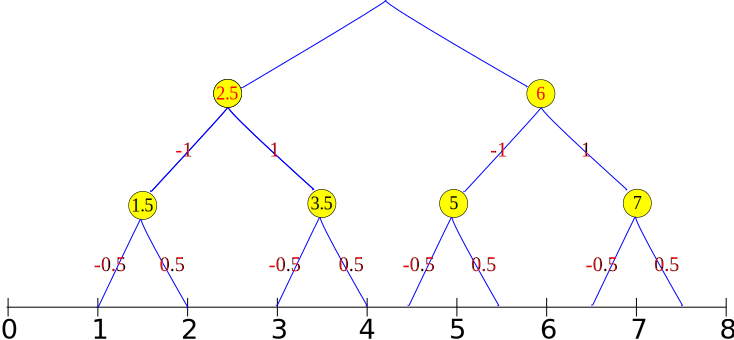
\includegraphics[width=0.75\textwidth]{thesis2/RVQ_trg_1_to_7_equivalentCVs.pdf}}
							\subfigure[Entanglement using a 2x4 encoder codebook.  The paths shown in bold will not be taken by any input data-point.  The shaded region is the stagewise partition class of the stage code-vector $\mu_{1,1}$~\cite{1993_JNL_RVQDSC_Barnes}.]{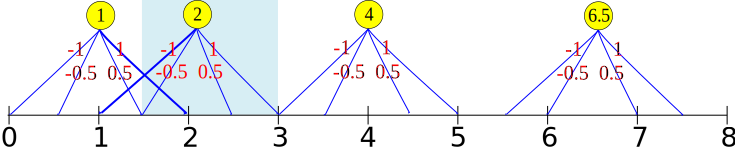
\includegraphics[width=0.75\textwidth]{thesis2/RVQ_trg_1_to_7_equivalentCVs_2.pdf}}
							\caption{Training set $S_{trg}=\{1,2,3,4,5,6,7\}$.  Construction of equivalent code-vectors using encoder codebooks given in Table~\ref{table:Exp1_encoder}.  In both cases shown above, the encoder codebook is exactly the same as the decoder codebook.  In the 3x2 case, the tree is unentangled since the equivalent partitions in $\mathbb{R}$ are connected regions~\cite{1992_JNL_RVQ_Barnes}.  In the 2x4 case, there is mild entanglement.}
							\label{fig:RVQ_entanglement_tree}
							\end{figure}

							\begin{figure}
							\centering
							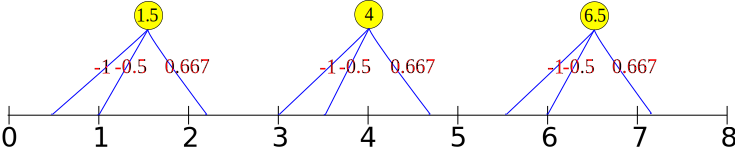
\includegraphics[width=0.75\textwidth]{thesis2/RVQ_trg_1_to_7_equivalentCVs_3.pdf}
							\caption{Training set $S_{trg}=\{1,2,3,4,5,6,7\}$.  Unentangled tree using a 2x3 encoder codebook.  Construction of equivalent code-vectors using encoder codebooks given in Table~\ref{table:Exp1_encoder}.  In both cases shown above, the encoder codebook is exactly the same as the decoder codebook.  In the 3x2 case, the tree is unentangled since the equivalent partitions in $\mathbb{R}$ are connected regions~\cite{1992_JNL_RVQ_Barnes}.  In the 2x4 case, there is mild entanglement.}
							\label{fig:RVQ_entanglement_tree}
							\end{figure}

The entanglement inhibits even placement of equivalent code-vectors, thereby increasing distortion.
Also notice that encoder and decoder codebooks are the same except for the 2x3 case.  Using the encoder codebook, the reconstruction rms error at the output of the first stage is 0.6547.  A slightly higher rms error of 0.7557 is achieved using the decoder codebook.   Table~\ref{table:Exp2_detailed_computations} gives detailed computations for code-vectors picked at every stage, reconstructions, errors, etc for the 2x3 encoder codebook.  

The actual rms errors as reported by gen.exe as given in Appendix~\ref{Exp1_gen_stat} and plotted in Figure~\ref{fig:RVQ_8x3_trg_1_to_7} are 0.6547 and 0.1543 respectively.


\begin{table}
\centering
\subtable[3x{\color{red}\textbf 2}]{\begin{tabular}{|c|c|}\hline 
2.5  & 6\\
-1  & 1\\
-0.5  & 0.5\\\hline
\end{tabular}}\hspace{0.2in}
\subtable[2x{\color{red}\textbf 3}]{\begin{tabular}{|c|c|c|}\hline
1.5 & 6.5 & 4\\
-1 & 0.667 & -0.5\\\hline
\end{tabular}}\hspace{0.2in}
\subtable[2x{\color{red}\textbf 4}]{\begin{tabular}{|c|c|c|c|}\hline
1 & 6.5 & 4 & 2\\
-1 & 1 & -0.5 & 0.5\\\hline
\end{tabular}}\hspace{0.2in}
\subtable[2x{\color{red}\textbf 5}]{\begin{tabular}{|c|c|c|c|c|}\hline
1 & 6.5 & 4.5 & 2 & 3\\
-0.5 & 0.5 & 0 & 0 &0\\\hline
\end{tabular}}\hspace{0.2in}
\subtable[2x{\color{red}\textbf 6}]{\begin{tabular}{|c|c|c|c|c|c|}\hline
1 & 6.5 & 4 & 2 & 3 &5\\
-0.5 & 0.5 & 0 & 0 &0 &0\\\hline
\end{tabular}}\hspace{0.2in}
\subtable[1x{\color{red}\textbf 7}]{\begin{tabular}{|c|c|c|c|c|c|c|}\hline
1 & 7 & 4 & 2 & 3 &5 &6\\\hline
\end{tabular}}
\hspace{0.2in}
\subtable[1x{\color{red}\textbf 8}]{\begin{tabular}{|c|c|c|c|c|c|c|c|}\hline
1 & 7 & 4 & 2 & 3 &5 &6&0\\\hline
\end{tabular}}
\caption{Experiment 1, RVQ \emph{encoder} codebooks with increasing code-vectors per stage, $m$~=~{\color{red}\textbf {2, 3, 4, 5, 6, 7, 8}}.  As $m$ goes up for a given training set, the number of stages $q$ falls.}
\label{table:Exp1_encoder}
\end{table}

\begin{table}
\centering
\subtable[3x{\color{red}\textbf 2}]{\begin{tabular}{|c|}\hline
same as encoder\\codebook\\\hline
\end{tabular}}\hspace{0.2in}
\subtable[2x{\color{red}\textbf 3}]{\begin{tabular}{|c|c|c|}\hline
1 & 6 & 4\\
-1 & 1 & 0\\\hline
\end{tabular}}\hspace{0.2in}
\subtable[3x{\color{red}\textbf 4}]{\begin{tabular}{|c|}\hline
same as encoder\\codebook\\\hline
\end{tabular}}\hspace{0.2in}
\subtable[3x{\color{red}\textbf 5}]{\begin{tabular}{|c|}\hline
same as encoder\\codebook\\\hline
\end{tabular}}\hspace{0.2in}
\subtable[3x{\color{red}\textbf 6}]{\begin{tabular}{|c|}\hline
same as encoder\\codebook\\\hline
\end{tabular}}\hspace{0.2in}
\subtable[3x{\color{red}\textbf 7}]{\begin{tabular}{|c|}\hline
same as encoder\\codebook\\\hline
\end{tabular}}\hspace{0.2in}
\subtable[3x{\color{red}\textbf 8}]{\begin{tabular}{|c|}\hline
same as encoder\\codebook\\\hline
\end{tabular}}
\caption{Experiment 1, RVQ \emph{decoder} codebooks with increasing code-vectors per stage, $m$~=~{\color{red}\textbf {2, 3, 4, 5, 6, 7, 8}}.}
\label{table:Exp1_decoder}
\end{table}



							\begin{figure}
							\centering
							\includegraphics[width=0.75\textwidth]{thesis2/RVQ_8x3_trg_1_to_7.pdf}
							\caption{Experiment 1, results for 2x3 RVQ.  eRMSE=\{0.6547, 0.1543\} for stages 1 and 2, and dRMSE=\{0\} for stage 2, as reported by gen.exe for 2x3 RVQ (Appendix~\ref{Exp1_gen_stat}).  The training set is $S_{trg}=\{1,2,3,4,5,6,7\}$.}
							\label{fig:RVQ_8x3_trg_1_to_7}
							\end{figure}


\begin{table}[t]
\scriptsize
\centering
\begin{tabular}{|l||c|c|c|c|c|c|c|}\hline 
\textbf{Test point} $\rightarrow$                             & \textbf{1}  &\textbf{2} &\textbf{3}   &\textbf{4}   &\textbf{5} &\textbf{6} &\textbf{7} \\\hline
\textbf{selected code-vector index at stage 1 (XDR)} $\rightarrow$ & 1     &  1   &  3   &  3   &  3   &  2     & 2 \\
\textbf{selected code-vector index at stage 2 (XDR)} $\rightarrow$ & 3     & 2     & 1   &  3   &  2   &  3     & 2 \\\hline\hline
\textbf{encoder: selected code-vector at stage 1} $\rightarrow$& 1.5     &1.5           &  4   &  4           &  4             &  6.5     & 6.5 \\
\textbf{encoder: selected code-vector at stage 2} $\rightarrow$& -0.5     & 0.6667     & -1   &  -0.5       &  0.6667   &  -0.5     & 0.6667 \\\hline
\textbf{encoder: recon. error after stage 1} $\rightarrow$& \color{blue}0.5  & \color{blue}0.5   &  \color{blue}1     &   0   &   \color{blue}1   &   \color{blue}0.5 & \color{blue}0.5 \\
\textbf{encoder: recon. error after stage 2} $\rightarrow$ & 0   &  \color{darkgreen}0.1667     &  0   &\color{darkgreen}\textbf{0.5}&   \color{darkgreen}0.3333    &   0   & \color{darkgreen}0.1667 \\\hline
\textbf{encoder: reconstructed output} $\rightarrow$             & 1         & 2.1667     & 3   & 3.5         &  4.6667   &  6         & 7.1667 \\\hline\hline
\textbf{decoder: selected code-vector at stage 1} $\rightarrow$& 1     &1           &  4   &  4           &  4             &  6     & 6 \\
\textbf{decoder: selected code-vector at stage 2} $\rightarrow$& 0     & 1     & -1   &  0       &  1   &  0     & 1 \\\hline
\textbf{decoder: recon. error after stage 1} $\rightarrow$        & 0       & 1     & 1   & 0         &  1   &  0         & 1 \\
\textbf{decoder: recon. error after stage 2} $\rightarrow$        & 0       & 0     & 0   & 0         &  0   &  0         & 0 \\\hline
\textbf{decoder: reconstructed output} $\rightarrow$             & 1         & 2     & 3   & 4         &  5   &  6         & 7 \\\hline
\end{tabular}
\caption{Experiment 1, computations for 2x3 RVQ.  Encoder rms error at the output of the first stage is {\color{blue}$\sqrt \frac{4(0.5^2) + 2(1^2)}{7} = \sqrt\frac{3}{7} = 0.6547$}, while the error at the output of the second stage is {\color{darkgreen}$\sqrt \frac{2(0.1667^2) + 0.3333^2}{7} = \sqrt\frac{0.1667}{7} = 0.1543$}.  Notice that in this second computation, we've omitted using 0.5, shown in boldface in the table, since the encoder error for data point 4 after the first stage has already reached 0, and an intelligent encoder should factor this into rms error computations.  These numbers match eRMSE as reported by gen.exe as shown in Figure~\ref{fig:RVQ_8x3_trg_1_to_7}.}
\label{table:Exp1_detailed_computations}
\end{table}




\clearpage
\newpage
\normalsize
\bibliographystyle{ieee}
\bibliography{MyCitations}
\end{document}